% ----------------------------------------------------------------------------
% Copyright (c) 2016 by Burkhardt Renz. All rights reserved.
% Die Vorlage für eine Abschlussarbeit in der Informatik am Fachbereich
% MNI der THM ist lizenziert unter einer Creative Commons
% Namensnennung-Nicht kommerziell 4.0 International Lizenz.
%
% Id:$
% ----------------------------------------------------------------------------

\chapter{Evaluierung}
\label{chapter:Evaluierung}
In diesem Kapitel werden die Prozesse beschrieben, die durchgeführt wurden, um die Implementierung und die erhaltenen Ergebnisse zu evaluieren. In \cref{section:Anforderungserfüllung} wird die Traktorimplementierung auf ihre Einhaltung der Anforderungen  untersucht. In \cref{section:Umsetzung der Designziele} werden die Designziele herangezogen und auf ihre Gegebenheit in der Tracingbibliothek überprüft. Das Open-Source Projekt \textbf{Jaeger} wird als Vergleichswerkzeug in den folgenden Abschnitten herangezogen. Jaeger ist eine auf der OpenTracing API basierenden \emph{state-of-the-art} Distributed Tracing Implementierung. Sie setzt die aktuellsten Erkenntnisse der Distributed Tracing Gemeinschaft um. Dabei wird in \cref{section:Bereitstellung der Traktorentwicklungsumgebung} die Bereitstellung der Testumgebung, in Hinsicht auf beide Werkzeuge, diskutiert. Die Bereitstellungsunterschiede beider Werkzeuge werden aufgezeigt. In \cref{section:Ergebnissvergleich} werden die Ergebnisse der Spangenerierung verglichen. Zuletzt werden die präsentierten Visualisierungansätze diskutiert. Es wird ein Vergleich zu dem Visualisierungsansatz der Jaeger UI durchgeführt.

\section{Anforderungserfüllung}
\label{section:Anforderungserfüllung}

Es ist eine Analyse durchzuführen, bei der die erhobenen Daten interpretiert werden. Die daraus gewonnenen Informationen sollen die End-zu-End Latenz einer Anfrage durch ein verteiltes System und die Generierungszeit eines Frames, welches durch die Unity Anwendung generiert wurde, darstellen. 

Die Implementierungsphase erfolgte nach dem Softwareentwicklungskonzept des \gls{tddGlossar}. Test-driven development ist ein Software Entwicklungskonzept, dass darauf basiert, kurze Iterationsphasen, durch die Implementierung von Tests und anschließender Funktionalitätsumsetzung, durchzuführen. Die Tests sollen den Anforderungen entsprechen, die an die Funktion gestellt werden. Die Mitentwicklung der Testbasis ermöglicht eine sich stetig verbessernde Abdeckung der Funktionsfähigkeit der Bibliothek. Auch eine anschließende Projektbereitstellungsautomatisierung wird damit erleichtert. Es wird also verhindert, dass sich technische Schulden anhäufen.

Die Anforderungen der Funktionalitäten ist anhand der Implementierungen und der Tests gegeben. Das gesamte Projekt ist dementsprechend der Bachelorarbeit beigefügt. Ein Ausschnitt aus den Tests vermittelt den grundsätzlichen Aufbau.

\begin{minipage}[]{\textwidth}
	\begin{lstlisting}[frame=trBL]
	[TestMethod]
	public void StartActive()
	{
	string expectedOperationName = "Testoperation";
	Tracer tracer = new Tracer();
	ISpanBuilder builder = tracer.BuildSpan(expectedOperationName);
	IScope scope = builder.StartActive();
	string[] actualSpanFields = scope.Span.ToString().Split(";");
	
	Assert.AreEqual(scope.Span, tracer.ActiveSpan);
	Assert.AreEqual(scope.Span, tracer.ScopeManager.Active.Span);
	Assert.AreEqual(tracer.ActiveSpan, tracer.ScopeManager.Active.Span);
	}
	\end{lstlisting}
	\captionof{lstlisting}{Unit-Test der Spanbuilder Klasse}
	\label{listing:Unit-Test der Spanbuilder Klasse}
\end{minipage}

Der StartActive Test, testet die Funktion \emph{StartActive} der SpanBuilder Klasse. Dabei wird ein Scope initialisiert, der einen Span beinhaltet. Der Span wird aktiviert und mit dem Span verglichen, der in dem Scopemanager verwaltet wird. Bei übereinstimmenden Werten der Felder, ist der Test bestanden und die Funktion entspricht den Anforderungen, die an diese gestellt werden.

Die Anforderung der End-zu-End Latenz und die Anforderung der Bestimmung der Generierungszeit eines Frames werden durch das Datenmodell erfüllt. Durch die Führung von \emph{Datetime} Objekten innerhalb der Spans, lassen sich Zeitspannen bestimmen, die ein Event einnimmt. Die Differenz aus Endzeit und Startzeit ergibt die Zeitspanne der Framegenerierung, da der Prozess der Framegenerierung durch einen Span darstellbar ist. Die End-zu-End Latenz ergibt sich aus dem hierarchisch am höchsten angeordneten Span eines Trace und den darüber hinaus, falls vorhanden, folgenden Spans, die den Beziehungstypen \emph{follows-from} besitzen. Die Differenz der Startzeit des ersten Spans und der Endzeit des letzten Spans ergibt die End-zu-End Latenz, die durch die Anfrage entsteht.

Die Rahmenbedingung der eingeschränkten Nachrichtenmodifikation ist durch die Umsetzung des Konzept der Kontextpropagierung mittels dem Registry-Service eingehalten. Die Kommunikationswege der Anwendungen werden dadurch nicht beansprucht.


\section{Umsetzung der Designziele}
\label{section:Umsetzung der Designziele}

Die Umsetzung der Designziele nahm Einfluss auf diverse Architekturentscheidungen. Eines dieser Entscheidungen ist die Wahl der Entwicklungssprachen. Die Tracingbibliothek ist in der Sprache C\# implementiert. Besonders das Designziel der \textbf{Portabilität} unter Rücksichtnahme der verteilten Rendering-Anwendung, die in C\# und C++ implementiert ist. C\# ist ein sogenannter \emph{managed code}. Managed code bedeutet, dass die Ausführung des Programmcodes in einer verwaltet Umgebung durchgeführt wird. Die \gls{clrGlossar} ist eine solche verwaltete Umgebung. Unity unterstützt die Ausführung von managed code, ohne großen Aufwand und einer dementsprechend guten Portabilität, durch zum Beispiel, dass Einbinden von C\# Bibliotheken über dem den Packetmanager Nuget. Die Traktorbibliothek wird automatisiert über Nuget veröffentlicht. Die Einbindung der Bibliothek ist demzufolge einfach und das Aktualisieren entsprechend schnell. Für den Traktor Agenten wird die Programmiersprache Python verwendet. Diese bietet ähnliche Flexibilität. Python ist eine interpretierte Sprache, wodurch sie auf jedem System ausgeführt werden kann, solange der Interpreter verfügbar ist.
Das Designziel der \textbf{Verarbeitungskosten} wurde nur teilweise umgesetzt. Das Konzept der Traktor Registry  erhöht den Overhead der Anwendung. Das Alternativkonzept des Interceptors ist vielversprechender. Dieses verzichtet auf einen Service zur Kontextpropagierung und setzt auf Nachrichtenmodifikation über die Manipulation der Anwendungsnachrichten mit Betriebssystemfunktionalitäten. Das Designziel der \textbf{Benutzbarkeit} ist durch die Vorbildnahme der OpenTracing API gegeben. Es wurden nur geringfügig Funktionalitäten hinzugefügt, damit das Konzept der Registry umgesetzt werden konnte. Die Ausdrucksweise zur Generierung von Traces ist gleich und entsprechend bewährt.



\section{Bereitstellung der Traktorentwicklungsumgebung}
\label{section:Bereitstellung der Traktorentwicklungsumgebung}

In diesem Kapitel werden die Prototypen einer verteilten Umgebung bereitgestellt. Die Bereitstellung ist ein zentraler Aspekt zur Erfüllung der Spezifikation der Traktorentwicklungsumgebung. Die Architektur hat nach \textbf{TE}.1 und \textbf{TE}.2 ein verteiltes System abzubilden. \textbf{TE}.1 ist durch die Architektur erfüllt. Es sind zwei Webserver implementiert, die miteinander kommunizieren und es ermöglichen, die Funktionalitäten der Instrumentalisierungsbibliothek zu nutzen und ihre Ergebnisse darzustellen.\textbf{TE}.2 spezifiziert, dass die Traktorentwicklungsumgebung auf einem Hostsystem läuft. Dabei soll trotzdem eine Verteilung der Komponenten des Systems gegeben sein. Dies ist durch die Anwendungskapselung mittels \emph{Container} gewährleistet. Ein Container beinhaltet eine Anwendungen, die benötigten Abhängigkeiten der Anwendung und Konfigurationsdateien. Die Sammlung der Container kommunizieren über Netzwerke miteinander. Die Infrastruktur wird mit \emph{Docker} umgesetzt. In dem Kontext der Softwarebereitstellung, ist Docker eine Sammlung von Open-Source Werkzeugen, die eine leichtgewichtige Betriebssystemevirtualisierung ermöglichen. Durch eine Konfigurationsdatei wird eine Infrastruktur definiert. Dabei werden die Services und das Netzwerk erstellt und anschließend auf dem Hostsystem zugänglich gemacht. Die Docker Konfigurationsdatei beschreibt den in \cref{fig:Docker-Compose-Vis} dargestellten Infrastrukturaufbau. Auf dem Hostssystem werden vier Container erstellt, die sich in dem traktor-network befinden. Die Container sind vorher über eine \emph{Dockerfile}, also einer Datei, die den Bauprozess eines Containers beschreibt, zu bauen. Die Dockerfile, die für den Bauprozess genutzt werden soll, wird als Pfad in der Variable build beschrieben. Damit die Container auch von außerhalb des traktor-network ansprechbar sind, wird ein \emph{Portmapping} vorgenommen. Das Portmapping stellt eine Verbindung von Hostport zu Containerport her. Dadurch wird ein Kanal geschaffen, über den zum Beispiel der HTTP Klient eine Anfrage an das verteilte System stellen kann. Die \emph{network}-Variable weist einem Container ein Netzwerk zu, in dem es sich befinden soll. Über die \emph{enviroment}-Variable werden Umgebungsvariablen innerhalb des Containers gesetzt, auf die die Anwendung zugreifen kann. Dies ist eine Vorgehensweise, mit dem man Containerkonfiguration vornimmt. Die \emph{depens\_on}-Variable stellt sicher, dass die spezifizierten Container vorher erstellt werden, die für diesen Container zur Funktionsfähigkeit notwendig sind. Die \emph{cap\_add}-Variable ist für den Interceptor notwendig. Container sind im Normalfall isolierte Prozesse, die auf das Hostsystem nur eingeschränkt zugreifen können. Durch die cap\_add-Variable wird dem Container zusätzliche Rechte gegeben. In diesem Fall das Recht, auf die Netzwerkschnittstellen zugreifen zu können.
\begin{figure}[]
	\centering
	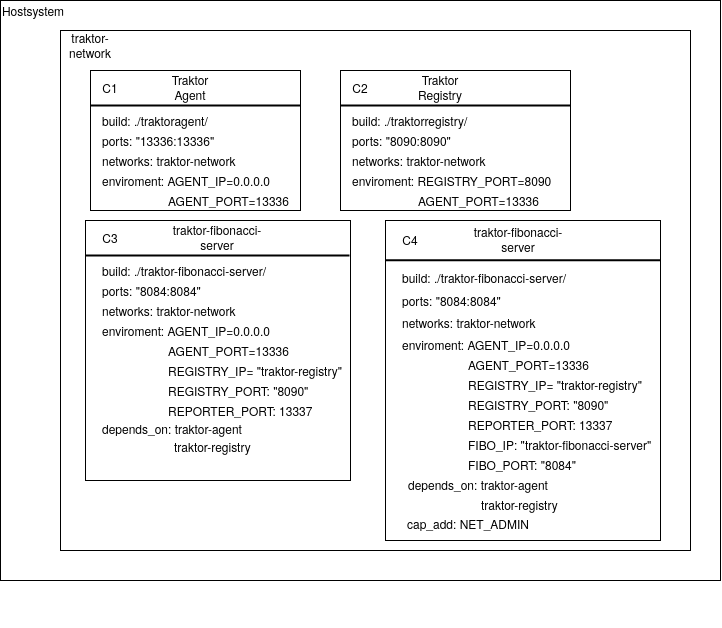
\includegraphics[scale=0.5]{img/Evaluation/Docker-Compose-Vis.png}
	\caption[Visualisierung der Docker Infrastruktur]{Darstellung der Docker Infrastruktur}
	\label{fig:Docker-Compose-Vis}
\end{figure}

\section{Ergebnissvergleich}
\label{section:Ergebnissvergleich}
Die Dateninterpretation wird auf Basis eines Datensatzes durchgeführt, welche aus der Traktorentwicklungsumgebung erhoben worden sind. 

Die Rohdaten sehen folgendermaßen aus:

\begin{minipage}[]{\textwidth}
	\begin{lstlisting}[frame=trBL]
	recieved message:  b'Server: Process Context;04/22/2020 09:29:00.1081 PM;S17JnBOXEmes;rtXWWLvE9XDg;child_of;04/22/2020 09:29:00.1097 PM{pi1a+hw7UuZN:child_of}'
	from:  ('172.22.0.5', 13337)
	recieved message:  b'CalculateFiboncacci;04/22/2020 09:29:00.1083 PM;S17JnBOXEmes;8glMa3Uu+jy2;child_of;04/22/2020 09:29:00.1084 PM{75buv+V8lmUn:child_of}'
	from:  ('172.22.0.5', 13337)
	recieved message:  b'CalculateFiboncacci;04/22/2020 09:29:00.1086 PM;S17JnBOXEmes;8V4vMLWZ2Ax/;child_of;04/22/2020 09:29:00.1086 PM{75buv+V8lmUn:child_of}'
	from:  ('172.22.0.5', 13337)
	recieved message:  b'CalculateFiboncacci;04/22/2020 09:29:00.1083 PM;S17JnBOXEmes;75buv+V8lmUn;child_of;04/22/2020 09:29:00.1087 PM{wngEpk/UsI3i:child_of}'
	from:  ('172.22.0.5', 13337)
	recieved message:  b'CalculateFiboncacci;04/22/2020 09:29:00.1089 PM;S17JnBOXEmes;wJ5dqhRUsV8h;child_of;04/22/2020 09:29:00.1089 PM{wngEpk/UsI3i:child_of}'
	from:  ('172.22.0.5', 13337)
	recieved message:  b'CalculateFiboncacci;04/22/2020 09:29:00.1083 PM;S17JnBOXEmes;wngEpk/UsI3i;child_of;04/22/2020 09:29:00.1090 PM{rtXWWLvE9XDg:child_of}'
	from:  ('172.22.0.5', 13337)
	recieved message:  b'Process Context;04/22/2020 09:29:00.0948 PM;S17JnBOXEmes;pi1a+hw7UuZN;child_of;04/22/2020 09:29:00.1188 PM'
	from:  ('172.22.0.4', 13338)
	\end{lstlisting}
	\captionof{lstlisting}{Tracerrohdaten aus der Traktorentwicklungsumgebung}
	\label{listing:Tracerrohdaten aus der Traktorentwicklungsumgebung}
\end{minipage}

Diese Rohdaten sind in dem Agenten eingetroffen, nachdem sie von den beiden Tracer reportet worden sind. Anhand der \cref{fig:TraktorEnv-ApplicationArchitecture} lassen sich sieben Spans erkennen, die zu einem Trace gehören. Es sind zwei Komponenten der Traktorentwicklungsumgebung instrumentalisiert. Zum einen ist das der Fibonacci-Caller und zum anderen der Fibonacci-Server. Der Caller nimmt die HTTP-Anfrage eines HTTP Klienten an und stellt wiederum selbst eine Anfrage mit dem Klientendaten an den Server. Der Span mit dem Operationsnamen \emph{Process Context} ist der zuletzt reportet Span. Gleichzeitig ist es der erste generierte Span. Dieser Span gehört zum Fibonacci-Caller. Nach der Kontextpropagierung generiert der Fibonacci-Server den Span mit dem Operationsnamen \emph{Server: Process Context}. Anschließend werden fünf weitere Spans erzeugt, die das Event der Berechnung der Fibonacci Zahl umfassen. Die Funktion zur Berechnung der Fibonacci Zahl ist rekursiv implementiert. Demzufolge ist der Operationsname \emph{CalculateFibonacci} gleich. Die gemessenen Zeiten der Spans werden nun genauer betrachtet. Der Hauptaugenmerk soll auf den Millisekunden liegen, da nur in diesem Zeitbereich Änderungen sichtbar sind.


\begin{table}[]
	\centering
	\resizebox{\textwidth}{!}{
		\begin{tabular}{|l|l|l|l|l|l|}
		\hline
		Operationsname          & Anfangszeit & Endzeit & Dauer  & Referenz:Beziehungstyp              & SpanID           \\ \hline
		Process Context         & .0948       & .1188   & 240 ms & Root                       & o86QWz3AWK0W     \\ \hline
		Server: Process Context & .1081       & 0.1097  & 1.6 ms   & \{pi1a+hw7UuZN:child\_of\} & rtXWWLvE9XDg+jy2 \\ \hline
		CalculateFiboncacci     & .1083       & 0.1090  & 0.7 ms  & \{rtXWWLvE9XDg:child\_of\} & wngEpk/UsI3i     \\ \hline
		CalculateFiboncacci     & .1083       & 0.1087  & 0.4 ms  & \{wngEpk/UsI3i:child\_of\} & 75buv+V8lmUn     \\ \hline
		CalculateFiboncacci     & .1083       & 0.1084  & 0.1 ms  & \{75buv+V8lmUn:child\_of\} & 8glMa3Uu+jy2     \\ \hline
		CalculateFiboncacci     & .1086       & 0.1086  & 0 ms    & \{75buv+V8lmUn:child\_of\} & 8V4vMLWZ2Ax/     \\ \hline
		CalculateFiboncacci     & .1089       & 0.1089  & 0 ms  & \{wngEpk/UsI3i:child\_of\} & wJ5dqhRUsV8h     \\ \hline
	\end{tabular}	
	}
	\caption{Spandaten der Traktorenviroment instrumentalisiert durch Traktor}
	\label{tab:Spandaten_Traktor}
\end{table}

\begin{table}[]
	\centering
	\begin{tabular}{|l|l|l|l|}
		\hline
		Operationsname          & Dauer 	\\ \hline
		Process Context         & 208.99ms  \\ \hline
		Server: Process Context & 0.8ms 	\\ \hline
		CalculateFiboncacci     & 0.2ms 	\\ \hline
		CalculateFiboncacci     & 0.19ms 	\\ \hline
		CalculateFiboncacci     & 0ms		\\ \hline
		CalculateFiboncacci     & 0m		\\ \hline
		CalculateFiboncacci     & 0ms		\\ \hline
	\end{tabular}
	\caption{Spandaten der Traktorenviroment instrumentalisiert durch Jaeger}
	\label{tab:Spandaten_Jaeger}
\end{table}
Die \cref{tab:Spandaten_Traktor} zeigt eine geordnete Liste von Spans die zu einem Trace, generiert in der Traktorentwicklungsumgebung, gehören. Die Hierarchie ist durch die Spanreferenz gegeben. Die Dauer ergibt sich aus der Differenz der Anfangs- und Endzeit. Die \cref{tab:Spandaten_Jaeger} zeigt eine Sammlung von Spans, die einen identischen Prozessablauf darstellen. Die Daten sind aus dem \emph{Jaeger User Interface} entnommen, die den Trace darstellen. Der Trace ist in \cref{fig:Trace_Dist} visualisiert. Die Visualisierung entstammt aus der Jaeger UI.
Der Unterschied der Gesamtzeit der beiden Traces liegt bei 30ms. Es ist zu erkennen, dass die Datenerhebung der Traktorinfrastruktur deutlich langsamer ist. Anhand dieser beiden Messungen ist die Traktorinfrastruktur 15\% langsamer, als die Jaegerinfrastruktur.

Auch zu erkennen sind die verschiedenen Messverfahren. Die Jaegerinstrumentalisierung verwendet die Startzeit des Root-Trace als Nullpunkt. Spans messen ihre Dauer von diesem Nullpunkt aus. Die Traktorinstrumentalisierung misst die Anfangszeit und Endzeit jedes Spans. Die Differenz ergibt die Dauer eines Spans.

Grundsätzlich ist durch das Darstellungsmodell der Spans eine Happens-Before Relation darstellbar. Die Ergebnisse zeigen diese Relationsdarstellung, von der Position ausgehen, dass die gemessenen Zeiten akkurat sind.  Die Traktorimplementierung implementiert keine Uhrsynchronisation. Aus diesem Grund ist eine Happens-Before Relation, wie in \cref{section:Problemstellung} beschrieben, nicht gegeben. Die Umsetzung einer Uhrsynchronisation, durch beispielsweise einem zusätzlichem Service, könnte eine korrekte Bildung von Happens-Before Relationen schaffen. Die Implementierung der Traktorbibliothek nutzt derzeit die jeweiligen Uhren der Komponenten des Systems, ohne eine Anpassung der gemessenen Zeiten oder einer globalen Uhr.

\section{Visualisierungvergleich von Traktor und Jaeger}
\label{section:Visualisierungvergleich von Traktor und Jaeger}

In diesem Kapitel wird ein Vergleich zwischen dem Traktor Visualisierungskonzept und der Jaeger UI Visualisierung gezogen. Hierbei wird das Visualisierungskonzept des dreidimensionalen Flammengraphs genutzt, um den Vergleich zu führen. Zuletzt wird eine kurze Erklärung bezüglich der Frame Galerie abgegeben.

 Die Visualisierung eines Trace durch die Jaeger UI besteht im Grunde aus einem zweidimensional dargestellten Koordinatensystem bei der die X-Achse die Zeit darstellt und die Y-Achse die Services mit ihren durchgeführten Operationen. Ein Span ist dementsprechend und wie in \cref{subsection:Span} genauer beschrieben, ein Objekt mit einem Operationsnamen, einer Zeitspanne, einem Identifikator innerhalb seines Trace und einer Identifikationsnummer zur Identifizierung des Trace, zu dem es gehört. Das Visualisierungskonzept von Traktor setzt im Design auf eine kavalierperspektivische Darstellung der Traces. Eine kavalierperspektive Darstellung ist eine schiefe Parallelprojektion. In dieser Darstellung werden die Ebenen, die parallel zur Horizontalen stehen, unverzerrt gezeichnet. Kanten die in die Tiefe gehen, werden in einem \ang{45}-Winkel gezeichnet. Dadurch entsteht ein räumlicher Eindruck der Visualisierung. Zudem baut sich die Hierarchie der Spans von unten nach oben auf. Eine gestrichelte Kante stellt Überschreitungen von Prozessgrenzen dar. Diese Überschreitungen sind somit alle instrumentalisierten Kommunikationswege der Anwendung. Beispiele der jeweiligen Visualisierungen eines gleichen Trace sind in \cref{fig:Trace_Dist} und in \cref{fig:Eval_TraktorEnv} dargestellt. 

Die Ähnlichkeiten der beiden Visualisierungen sind dahingehend gegeben, dass es jeweils eine Achse gibt, die die Zeit und die Services darstellt. Auch die Zeitspannen, die die einzelnen Spans einnehmen, sind in beiden Visualisierungen gegeben. Die Gesamtdauer des Trace ist in beiden Visualisierungen dargestellt. Die Darstellung der Zeitspannen bei großen Unterschieden ist in beiden Visualisierungen schwierig. Diverse Spans nehmen extrem viel Zeit ein und ziehen dementsprechend die Zeitleiste sehr lang.

Unterschiede sind vor allem in der Darstellung der Services aufzufinden. Bei der Jaeger UI Visualisierung sind die Services nur anhand des Servicenamen und Operationsnamen identifizierbar. Das Traktor Visualisierungskonzept setzt einen starken Fokus auf diese Unterscheidbarkeit. Dadurch wird dem Benutzer einen Vorstellung der Architektur gegeben. Das Traktor Visualisierungskonzept bietet eine Abstraktion von Rohdaten. Diese Abstraktion äußert sich dahingehend, dass dem Anwender nebenbei Informationen durch die Darstellungsform gegeben werden, die im Falle von Jaeger explizit geschrieben stehen müssen, ohne starken visuellen Eindruck, abgesehen von einer farblichen Unterscheidung. Ein weiterer Unterscheidungspunkt sind die eingetragenen Zeiten der Prozessübertritte. Das Traktor Visualisierungskonzept stellt die Zeiten von Prozessüberschreitungen durch eine gestrichelte Linie dar. Zudem wird der Zeitstempel von wichtigen Ereignissen, wie zum Beispiel dem Anfangszeitpunkt des Trace, dem Endzeitpunkt des Trace und die Zeitpunkte der Prozessüberschreitungen, eingetragen. Diese sind in der Visualisierung \cref{fig:Eval_TraktorEnv} als \textbf{t1}, \textbf{t2}, \textbf{t3} und \textbf{t4} dargestellt. Das Traktor Visualisierungskonzept hat Schwierigkeiten, sobald die Hierarchie sehr groß wird. Die Spanblockehöhe hat somit ein ähnliches Problem, wie die Zeitachse.

Aus dem Vergleich lässt sich schließen, dass beide Visualisierungskonzepte Ähnlichkeiten aufweisen, dabei aber ihre Stärken hervorheben. Die Stärken des Traktor Visualisierungskonzept liegt in der Unterscheidungsfähigkeit der Prozesse. Diese Unterscheidungsfähigkeit wird dadurch gegeben, dass Daten derart genutzt werden, dass diese in der Darstellungsform wiedergegeben werden, anstatt diese als Text zu platzieren. Auch die Kommunikationswege sind durch die Verwendung von visuellen Eindrücken, wie zum Beispiel der gestrichelten Linien, besser verpackt. Die Jaegervisualisierung legt Fokus auf große Datenmengen und Skalierbarkeit. Da die Skalierbarkeit ein erklärtes Nicht-Ziel ist, wie in \cref{section:Designziele} beschrieben, ist die ausführlichere Darstellung eine positive Eigenschaft des Traktor Visualisierungskonzepts.


Das Visualisierungskonzept der Frame Galerie ist eine spezialisierte Form der Jaeger UI Visualisierung. Die Frame Galerie ist in drei Ebenen aufgeteilt. Jede Ebene stellt ein Abstraktionslevel dar. Die unterste Ebene, beschrieben in \cref{subsection:Frame Galerie}, soll konzeptionell der Jaeger UI Visualisierung ähneln. Die mittlere und obere Ebene sorgen dafür, dass eine Auswahl an relevanten Informationen getroffen werden kann, die in der unteren Ebene detailliert dargestellt werden.

\begin{figure}[!ht]
	\centering
	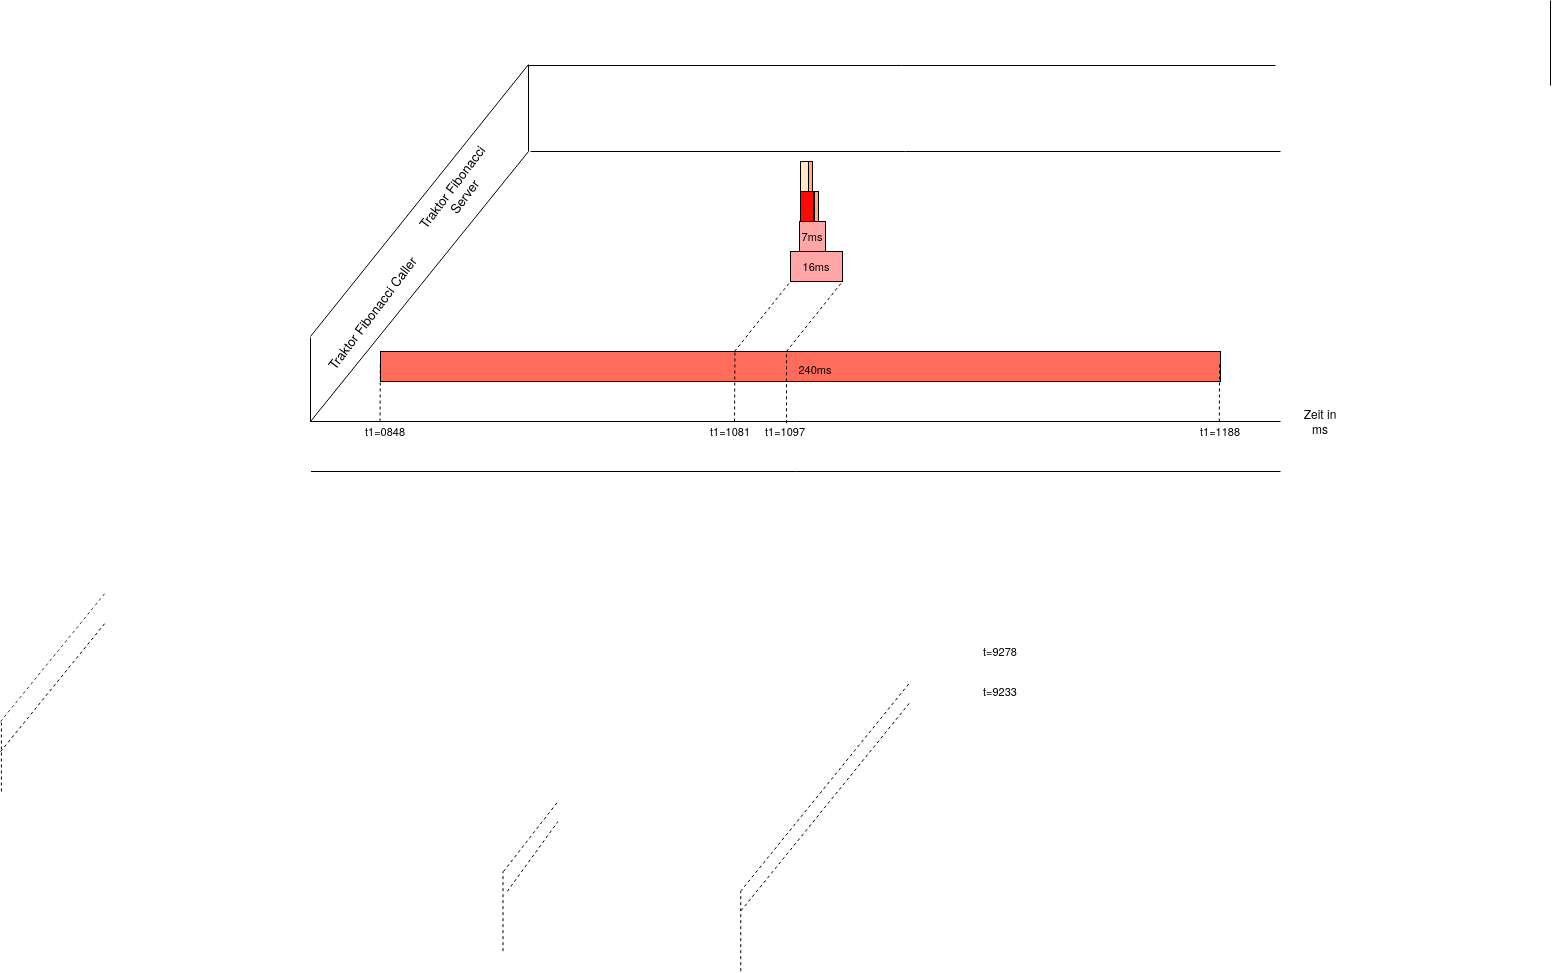
\includegraphics[scale=0.4]{img/Evaluation/Eval_TraktorEnv.png}
	\caption[Visualisierung eines Traktor-Trace]{Visualisierung eines Traktor-Trace}
	\label{fig:Eval_TraktorEnv}
\end{figure}


\begin{landscape}
	\begin{figure}
	%	\centering
		\hspace*{-130pt}
		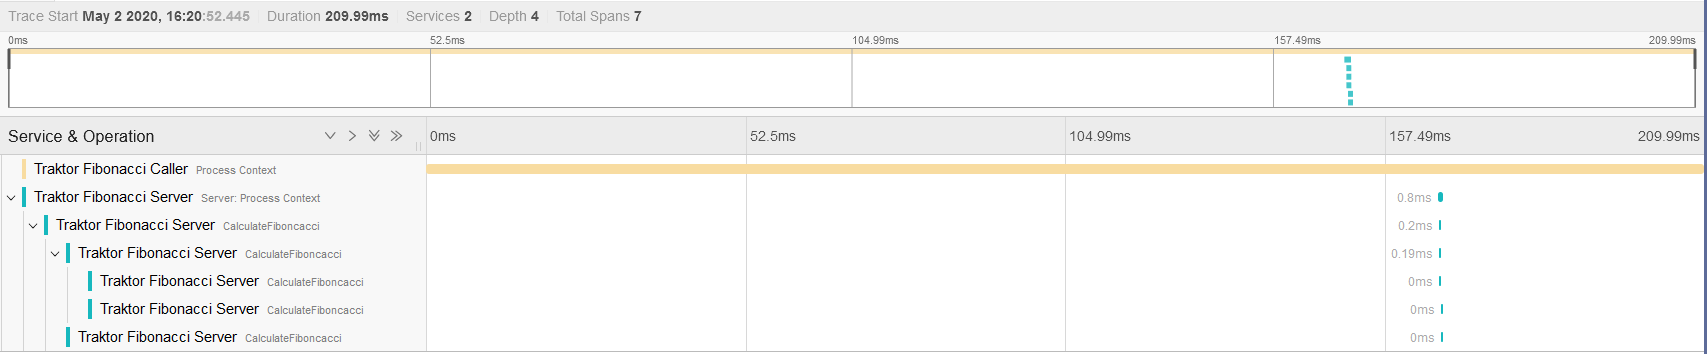
\includegraphics[scale=0.55]{img/Evaluation/Trace_Dist.png}
		\caption[Visualisierung eines Jaeger Trace durch Jaeger UI]{Visualisierung eines Jaeger Trace durch Jaeger UI}
		\label{fig:Trace_Dist}
	\end{figure}
\end{landscape}

% ----------------------------------------------------------------------------
